% meta.concepts: dry friction
% meta.tags: realistic
% acknowledge: Peter Seiler & Luke Melander graciously shared Spring 2019 course material
% source: 2019 P. Seiler AEM2011 HW 10

Professor Seiler is trying his hand at rappelling. He has chosen a cliff (AOB) which is inclined to the vertical as shown in the figure. It is known that $\theta = 80$ degrees and $\beta = 65$ degrees. It is also know that Professor Seiler weighs $750$ N. His CG is located at $162$ cm from his feet and he is holding the rope with his hands which are at a distance of $180$ cm from his feet as shown on the right. Let the coefficient of friction between his feet and the cliff wall be $\mu_s$.

Find:
\begin{enumerate}
  \item Tension in the rope.
  \item The minimum value of $\mu_s$ so that he does not slip and remains in equilibrium.
\end{enumerate}

\begin{figure}[ht!]
  \centering
  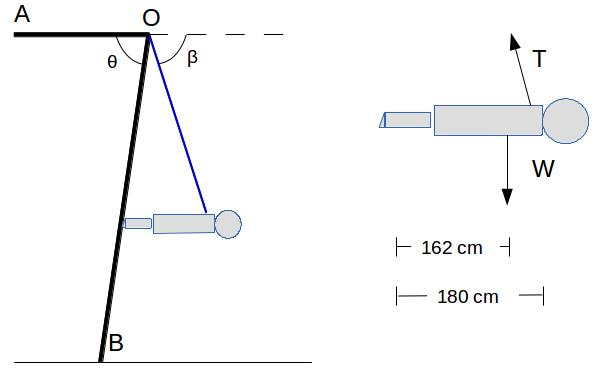
\includegraphics[width=0.4\textwidth,
	           height=0.3\textheight,
		   keepaspectratio]{fig.png}
\end{figure}

\iftoggle{flagSoln}{%
\vspace{.5cm}
\rule{\textwidth}{.4pt}
\vspace{.5cm}
\textbf{Solution:}
\begin{figure}[ht!]
  \centering
  \frame{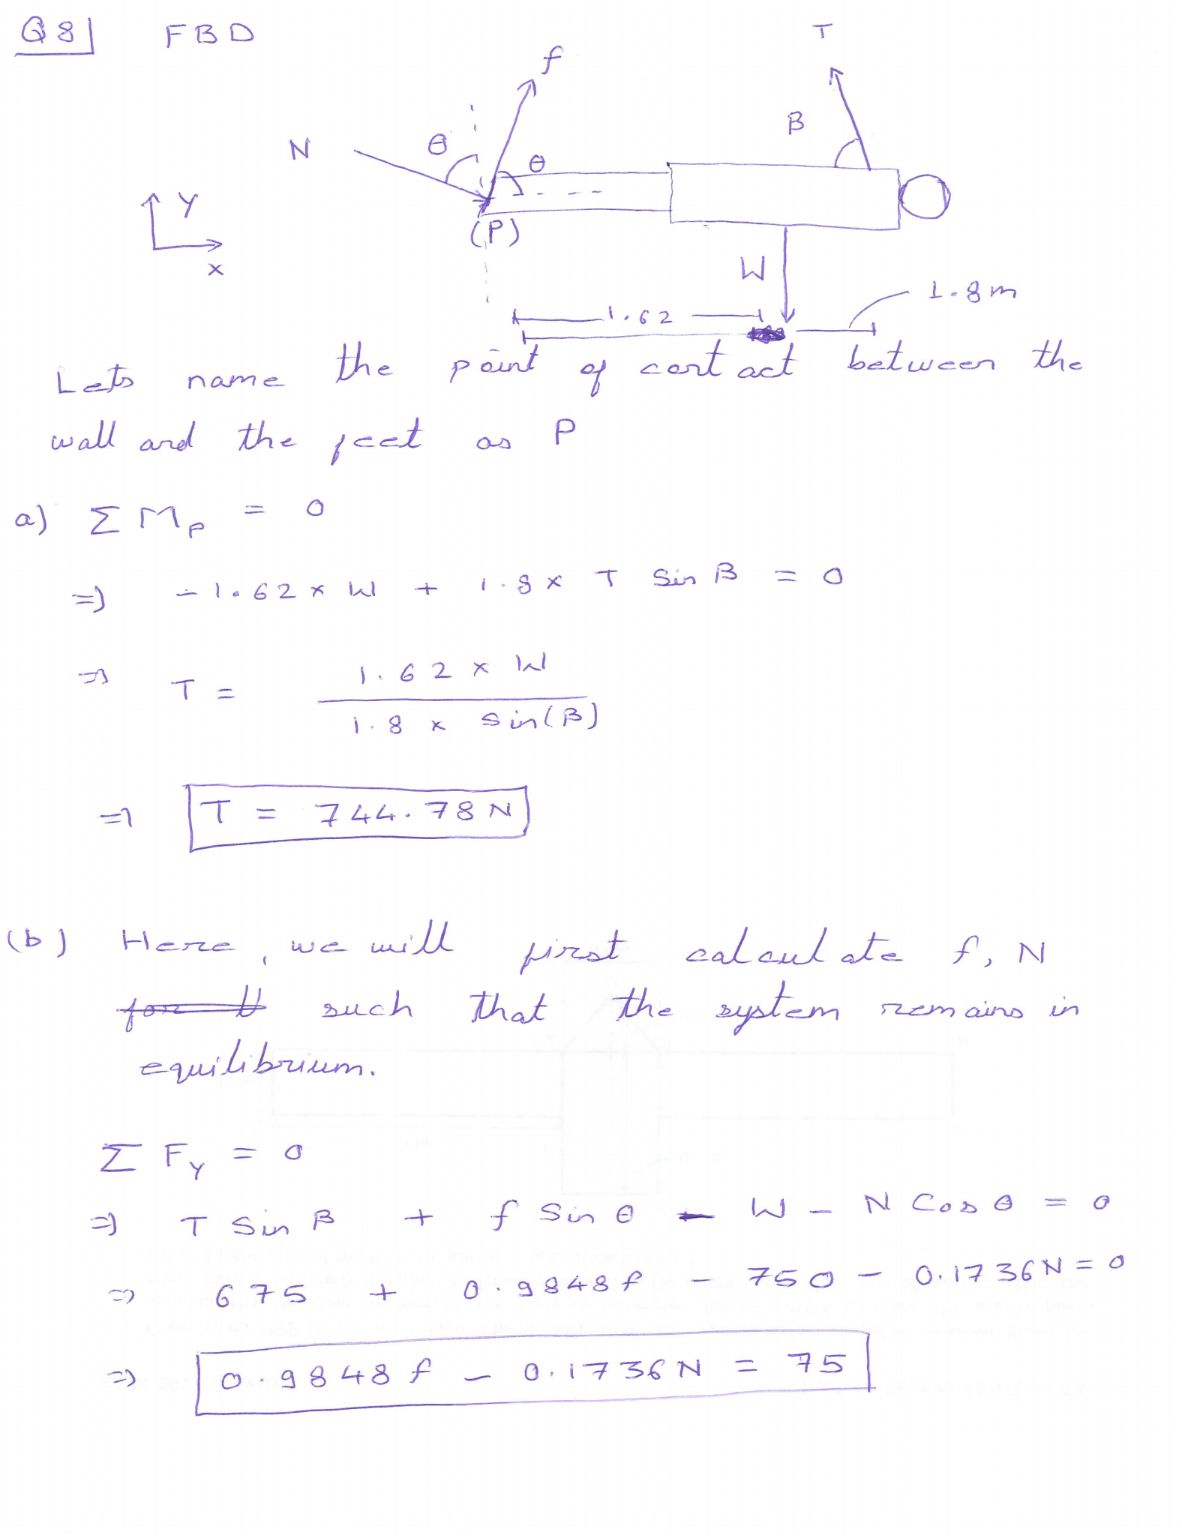
\includegraphics[width=0.9\textwidth,
	           height=0.4\textheight,
       keepaspectratio]{solna.png}}
  \frame{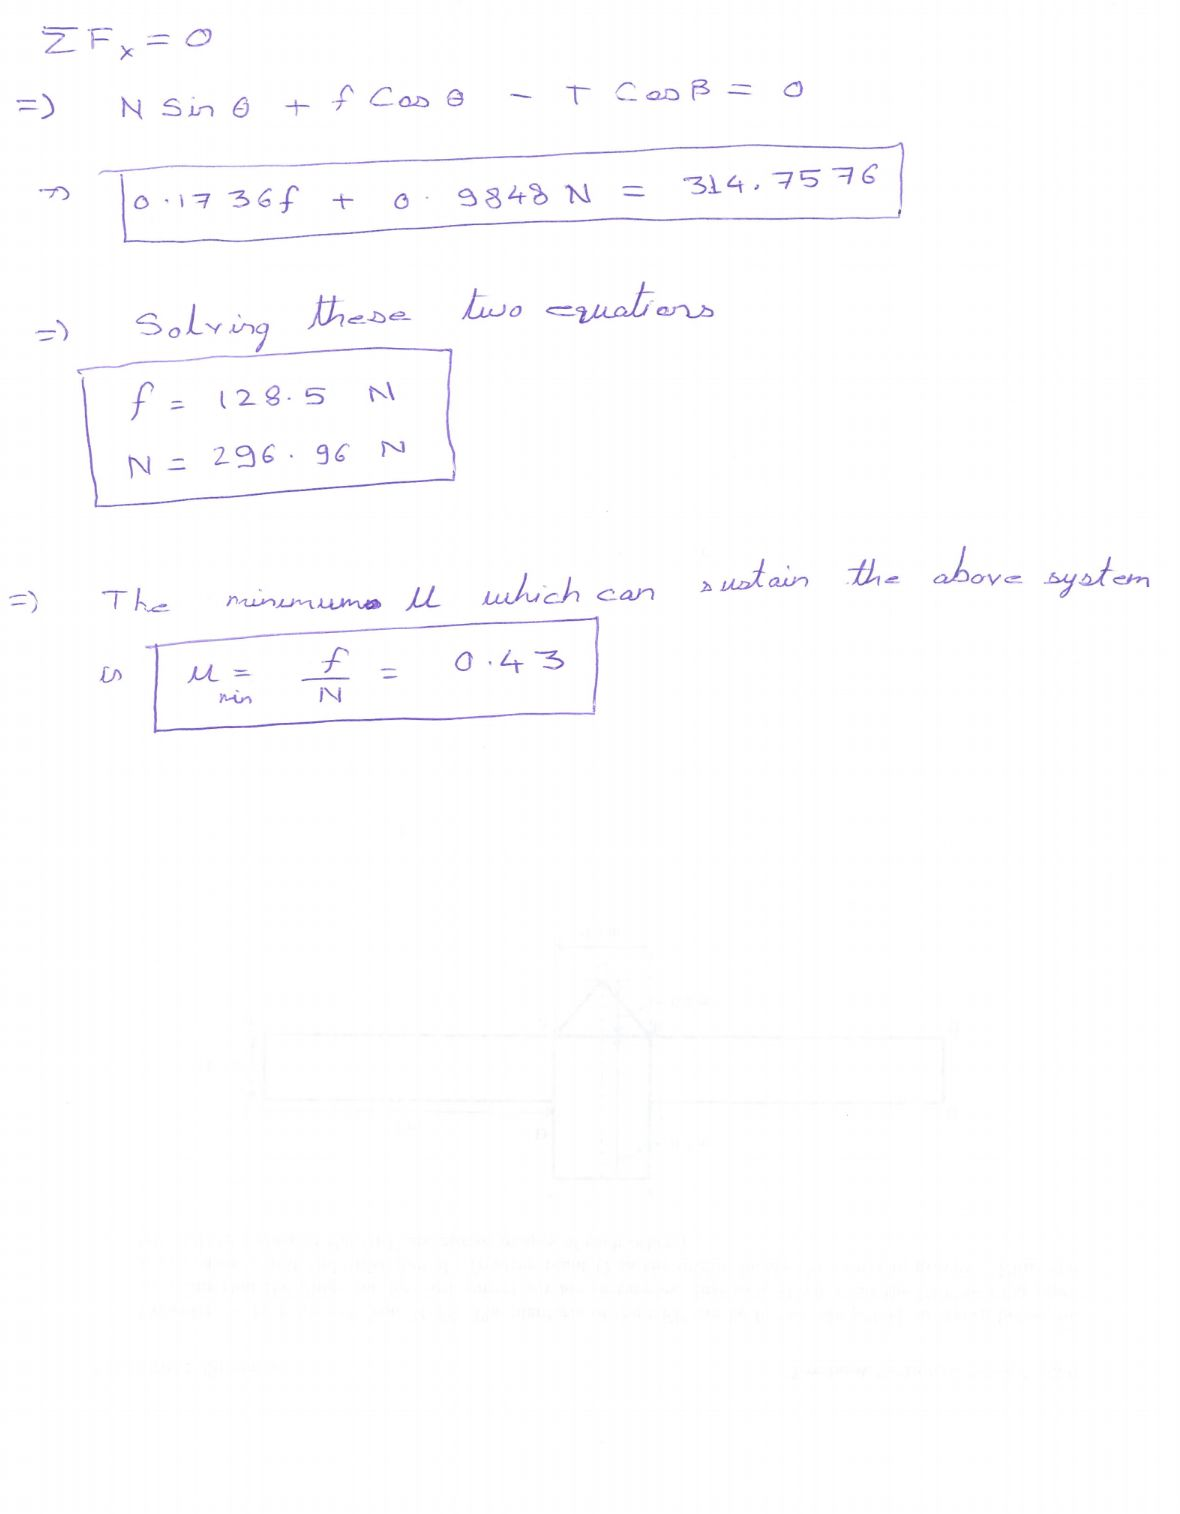
\includegraphics[width=0.9\textwidth,
	           height=0.4\textheight,
       keepaspectratio]{solnb.png}}
\end{figure}
}{%
}%
